\chapter{Overview}
\label{cha:intro}

\section{The major problem of physicians: time}
\label{sec:problem_doctors}

Physicians all over the world visit patients under time limitations. In addition, in developing countries like the Philippines\footnote{This work derives from a joint project between the University of Trento, the University of the Philippines and the Philippine
General Hospital \cite{johndocument}.}, there is not always a suitable doctor-population ratio (1:1000 is the optimal ratio according to the World Health Organization)\cite{johndocument}: thus, doctors in those places may be overloaded with work. Hence, the main problem of physicians is time. This obviously affects the way in which doctors examine patients, especially the anamnesis elicitation, which is the most time-consuming task during medical examinations.

\subsection{The anamnesis elicitation: a crucial but time-consuming task}

The anamnesis of a patient is the information gained by a physician by asking specific questions whose answers may be useful in formulating a diagnosis\cite{historytakingwiki}. This task, often called in medical jargon “history taking”, requires a long procedure because the physician does not have only to interview the patient and gather information about the history of their problem, but even write down a brief summary of the conversation in the patient’s record. This necessary bureaucracy is demanding and risks becoming all-embracing. For example, a research group monitoring 57 physicians in the United States observed that during the clinic day, physicians were spending 49.2\% of their clinical time on health records and desk work and only 27\% of their time with patients \cite{sinsky}. However, this task is fundamental: according to research, medical history provides in the 82.5\% of patients enough information to make an initial diagnosis of a disease \cite{hampton1975}.

The traditional way of interviewing the patient is not only long and demanding, but even sometimes incomplete. For instance, 134 primary care physicians observed that, during the study, only 59\% of essential history items were collected during history taking. Physicians were able to obtain relevant information about presenting symptoms and medications, but they often missed important information about related symptoms and medical history. This because a physician needs to remember a large number of questions and symptoms to have a complete and accurate history. Human memory is fallible and forgetting to ask some relevant questions during an interview might have a significant implication in patient management.\cite{johndocument}

\subsection{An alternative to the traditional anamnesis elicitation}

Therefore, it is for the aforementioned reasons that a new approach to anamnesis should be tried. Digitize this task is a possible solution which is time-saving for physicians and, at the same time, could provide a better history taking outcome. The ideal interaction model between this history taking program and the patient is a chat conversation. Basically, the patient, chatting, interacts with this conversational software, which has to understand and classify the presenting symptoms and, later, elicit symptoms and information useful for the diagnosis that the patient may have forgotten. A first obstacle towards an effective history taking dialogue system is identifying and classifying symptoms within a patient’s answer. This work is focused on it.

\section{What does identifying and classifying symptoms mean?}

This section is dedicated to present a high level view of the work and the two main abstract components of the code: the \textit{Symptom Identifier} and the \textit{Symptom Classifier}. 

\label{sec:identifying_classifying}
\subsection{Identifying symptoms}

Identifying symptoms within a patient's sentence means finding, inside the text of the sentence, every group of adjacent words that carry together a coherent symptom concept.

\begin{figure}[h]
\centering
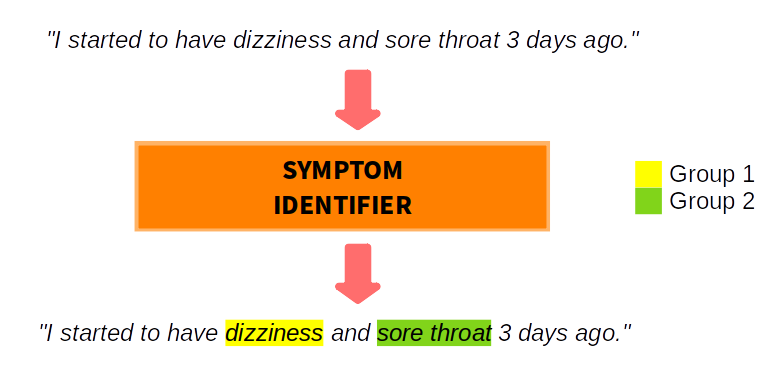
\includegraphics[width=12cm]{symptom_identifier}
\caption{The \textit{Symptom Identifier} seen abstractly.}
\medskip
\end{figure}
\newpage
These groups of words will then be mapped into precise symptoms contained in a symptom classification: they are named \textit{tokens for predictions} (TFPs for short).

\subsection{Classifying symptoms}
\label{sec:cla_symp}

Thus, the objective of the Symptom Classifier is to map correctly the previous \textit{tokens for predictions} into a list of specific symptoms. Each symptom inside the classification has an unique identifier called CUI (Concept Unique Identifier). The first character of a CUI is a \texttt{C} followed by seven digits.

\begin{figure}[h]
\centering
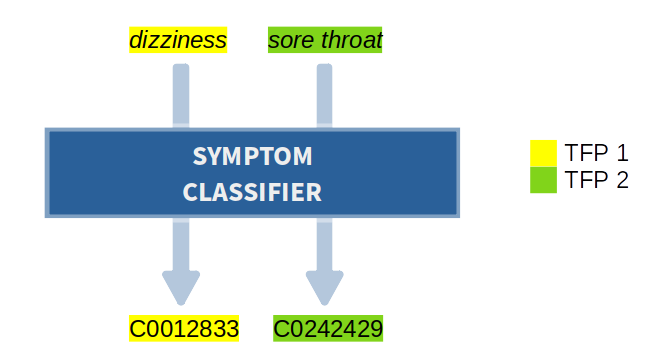
\includegraphics[width=10cm]{symptom_classifier}
\caption{The \textit{Symptom Classifier} seen abstractly.}
\medskip
\end{figure}

\subsubsection{The MEDCIN symptom classification}
MEDCIN is a medical terminology system developed by Medicomp Systems Inc. \cite{medcin}. It contains more than $300\,000$ clinical data elements encompassing symptoms, physical examinations, tests, diagnoses and therapies. What makes MEDCIN particularly fit for the purpose of this work is its nature of being a \textit{point of care} terminology system. This means that MEDCIN is intended to help clinicians in documenting clinical information while interacting with patients. Therefore, MEDCIN includes all the symptom concepts that a physician may need when summarizing a patient's problem. In addition, another positive aspect stands in its hierarchical organization: the symptoms are structured in a tree, and each child of a node is in a \textit{is-a} relationship with its father.

Although MEDCIN is copyrighted, it is inside the list of supported UMLS terminology systems. The Unified Medical Language System (UMLS) is a compendium of many controlled medical vocabularies and it is maintained by the US National Library of Medicine \cite{umls}. Academic users may access the UMLS free of charge for research purposes.

Encompassing MEDCIN, UMLS provides a mapping structure between it and any other terminology system supported by UMLS. This is positive because CUIs are codes which are transversal to all the vocabularies inside the UMLS.

\subsubsection{But why is  classifying symptoms necessary?}
\label{sub:whyclassifying}
Find an appropriate mapping for a \textit{token for prediction} is not a trivial task, mainly because reality is not easily classifiable; natural language in particular. However, mapping symptoms to a classification is useful especially for improving the quality of the chatbot. This because the long-term objective is not to understand the presenting symptoms (physicians, and, generally, every human, are very good at it) but ask clever questions to the patient in order to extract missing symptoms and, in general, useful information for the diagnosis. This could be done asking questions about related symptoms or reviewing the body systems (Review of Systems (ROS) is normal practice in history taking). For these reasons, a mapping to a standard symptom classification is essential.

\section{Brief description of methods}
\label{sec:brief_methods}

This section will briefly outline the methods that has been developed and the technologies that has been used. Then, chapter \ref{cha:methods} will deepen more into the details of the components listed below.

\subsection*{Symptom identifier}
The abstract component \textit{Symptom Identifier} is made up of three sub-components:
\begin{itemize}
  \item a \textit{Body Part Finder}. Its aim is to identify words that are common body parts inside the sentence. The purpose is to find them and later inform the next component about the body parts that appeared within the sentence;
  \item a \textit{Question Answering (QA) system}. The objective of this component is, given a set of questions, aswering them highlighting the parts of the sentence which respond to each question. This task is called \textit{Maching Reading Comprehension} and can be done with these two supported models:
    \begin{enumerate}
      \item \textit{BERT}, that stands for \textit{Bidirectional Encoder Representations from Transformers} \cite{bert}, finetuned on \textit{SQuAD} (a Reading Comprehension dataset developed by Stanford University) \cite{squad};
      \item \textit{R-NET}, an end-to-end neural networks model for Reading Comprehension developed by Microsoft  \cite{rnet};
    \end{enumerate}
  \item an \textit{Answer Interpreter}. In this stage the answers of the previous component (the \textit{QA system}) become \textit{tokens for predictions}: this prepares them for the vectorization.
\end{itemize}

\subsection*{Symptom classifier}
The abstract component \textit{Symptom Classifier} is made up of two sub-components:
\begin{itemize}
  \item a \textit{Vectorifier}. The purpose of this component is encoding a given sentence into an embedding which can be of two types:
  \begin{enumerate}
    \item \textit{GloVe} embeddings \cite{glove};
    \item \textit{BERT} embeddings;
  \end{enumerate}
  \item a \textit{Symptom Tree Mapper}. The aim of this component is returning, given the embedding of a \textit{token for prediction}, the CUI of the most similar symptom. Similarity is a suitable measure because both the \textit{tokens for predictions} and each symptom name can be vectorized; thus, for both of them, an internal representation is available.
\end{itemize}

\subsection*{Dataset}
\label{datasetintro}
Up to now, there are not any suitable datasets for this project; therefore, for the purpose of this work, it proved necessary scraping and tagging $336$ sentences extracted from posts of a medical forum \footnote{\url{https://www.doctorslounge.com/forums/}} \cite{doctorslounge}. In section \ref{sec:dataset} is described the process that was followed in order to create this dataset.

\section{Brief description of results}
\label{sec:brief_results}
As shown in chapter \ref{cha:results}, BERT is better than R-NET in identifying symptoms. As a matter of fact, using BERT, the percentage of correct tokens is $84.8 \%$, while, using R-NET it is of $70.4 \%$ ($+ 14.4 \%$ of improvement). BERT for QA outperforms R-NET even in other indices presented in section \ref{sec:eval_symptom_identifier}.

In section \ref{sec:evalsymptomclassifier}, any option of the Symptom Classifier is analyzed one by one: this means testing the model with different embedding types, if using or not the Body Part Finder and other options such as \textit{pruning}, filtering ``useless words'' and the minimum similarity threshold that will be treated in the corresponding section.

\section{Literature review}
This section will briefly outline the main state-of-the-art models related to this project.

At the moment, research is mainly focused on recognizing named entities within clinical texts; for example, these are: symptoms, tests, treatments, medications and chemical names. Hence, as shown in table \ref{tab:comparativeNER}, the available models are not specialized in classifying symptoms: they simply perform \textit{Named Entity Recognition} (NER).

An experimental comparison of different Machine-Learning approaches to medical entity recognition is presented in \cite{liu2017}. This work investigate the performance of LSTM (long-short term memory), a representative variant of RNN, on clinical entity recognition. It concludes that LSTMs perform only slightly better than Structured Support Vector Machines (SVM) on this task.

In addition, the publicly available recognition systems of symptoms are rare. This because of the diversity and complexity of symptom named entities in naming conventions and the lack of appropriate training corpora \cite{wei2016disease}. In order to avoid the first problem, this work proposes to map the symptoms identified in text to a medical standard classification (MEDCIN).
 
However, while symptom identification (i.e. recognition) has been recently investigated, symptom classification has not yet been studied. Nevertheless, as discussed in section \ref{sub:whyclassifying}, mapping symptoms towards a standard classification can be useful for eventual future components based on this work.

\hspace*{2in}
\begin{table}[h]
  \centering
  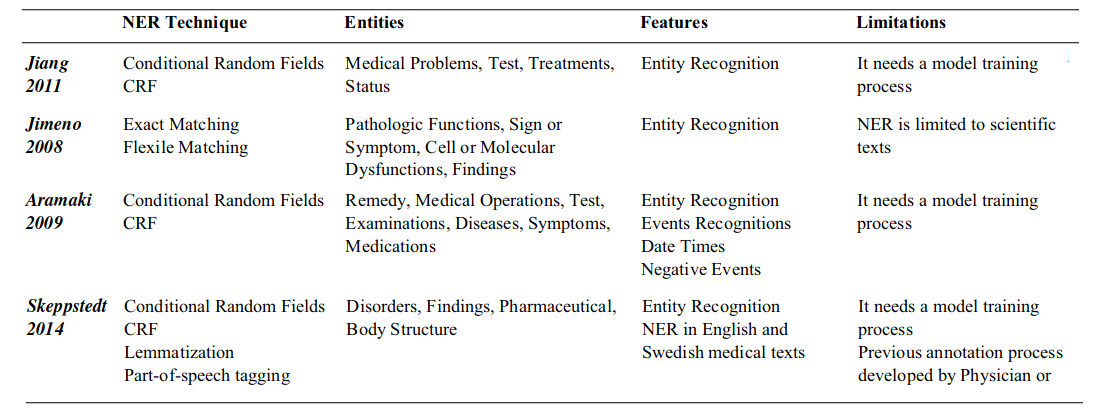
\includegraphics[width=17.5cm]{comparisonNER}
  \caption{Comparative analysis of various methods of NER in medical texts (Jiang et al. \cite{jiang2011}, Jimeno et al. \cite{jimeno2008}, Aramaki et al. \cite{aramaki2009} and Skeppstedt et al. \cite{skeppstedt2014}). Table taken from \cite{NERoverEHR}.}
  \label{tab:comparativeNER}
\end{table}

